

\section{FFTW and MPI}

\subsection{Library's}
The test programs we use to simulate the load a astronomy supercomputer endures rely on a few library's. The FFTW\footnote{Fastest Fourier In The West} and the OpenMPI\footnote{Message Passing Interface} library. \par The FFTW library is used for the fourier transformations, it has integrated support for multi threading which is what one of the test programs uses. And it also has support for MPI which is what the other FFT test program uses. \par The MPI library is used for the communication between the pi's, and requires some know how to properly install. But if you follow this install guide everything should work. 

\subsection{Setup}
For the MPI programs to work it is important that all pi's can ssh to each other, since this is how they communicate. So they all need to be connected to the same network. In our setup two network switches are used to connect all the pi's to a router via ethernet cables, as shown on figure \ref{fig: Pi's with router}.
\begin{figure}[h!]
    \centering
    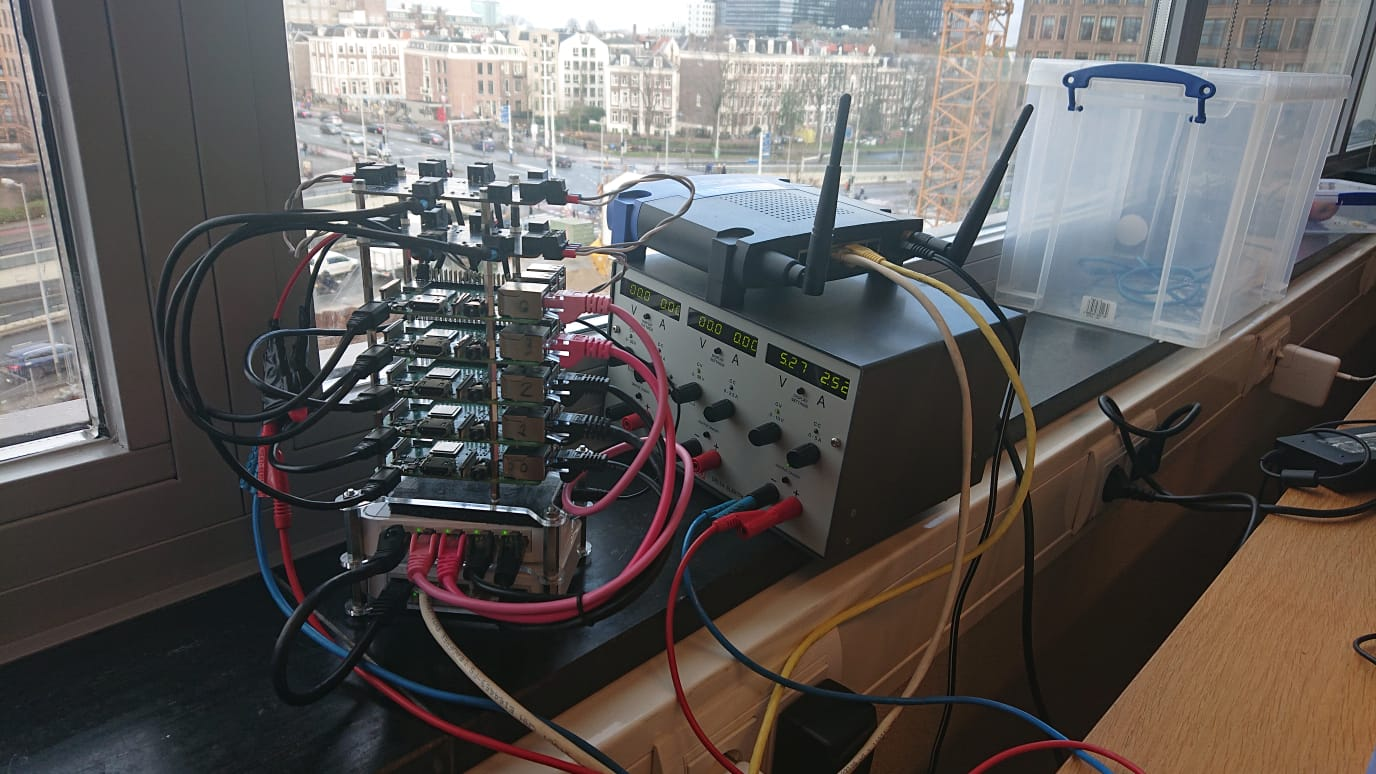
\includegraphics[width=\linewidth]{images/Pi_with_router.jpeg}
    \caption{Raspberryi pi's connected to router}
    \label{fig: Pi's with router}
\end{figure}

The process of giving each pi ssh access to each other has sadly not yet been automated and will have to be done manually. Each pi needs to have a ssh key and it's ID copy'd to all other pi's. To do this use the following commands:

\code{ssh-keygen}

followed up by,

\code{ssh-copy-id pi@[ip adress of each pi].local\\}


I've made a table you can use to keep track of which pi has ssh access to which other pi.
\begin{table}[h!]
\centering
\begin{tabular}{l|l|l|l|l|}
\cline{2-5}
                                          & pi-0 & pi-1 & pi-2 & pi-3 \\ \hline
\multicolumn{1}{|l|}{ssh-keygen}          &      &      &      &      \\ \hline
\multicolumn{1}{|l|}{ssh-copy-id to pi-0} &      &      &      &      \\ \hline
\multicolumn{1}{|l|}{ssh-copy-id to pi-1} &      &      &      &      \\ \hline
\multicolumn{1}{|l|}{ssh-copy-id to pi-2} &      &      &      &      \\ \hline
\multicolumn{1}{|l|}{ssh-copy-id to pi-3} &      &      &      &      \\ \hline
\end{tabular}
\end{table}

The ip adress of each pi is also needed for the machinefile, this is a file that MPI uses to know which "machines" it has avalible. 
A machinefile looks like this, Listing \ref{lst: machinefile}

\begin{lstlisting}[caption={Machinefile for MPI}\label{lst: machinefile}, frame=single]
pi@192.168.3.11 node0
pi@192.168.3.16 node1
pi@192.168.3.5  node2
pi@192.168.3.37 node3
\end{lstlisting}

And is located in the directory of the executable that uses MPI. (it can be located elsewhere but in the directory itself is easiest in my opinion) 

\subsection{Installation}

The install process has been automated using ansible scripts and is therefore very straightforward, we created a host group so the command can be sent to all pi's at once. 

To install the library's, make sure you have all the pi's that you want to run the programs on in your ansible hosts file. In our case this file was located in  \code{/etc/ansible/hosts} and contained the following lines:\newline 
 \code{[sfs]\newline
raspberrypi-0.local ansible\_user=pi\newline
raspberrypi-1.local ansible\_user=pi\newline
raspberrypi-2.local ansible\_user=pi\newline
raspberrypi-3.local ansible\_user=pi\newline
}

This means that you can run the playbook file \code{ansible/ansible\_install\_fftw.yaml} with the following command: 
\code{ansible-playbook ansible/ansible\_install\_fftw.yaml -l sfs}.

After this you can run the playbook \code{ansible/ansible\_install\_Test\_programs.yaml} with the following command: \newline \code{ansible-playbook ansible/ansible\_install\_Test\_programs.yaml -l sfs}.
